% final_report.tex — Báo cáo cuối kỳ chuẩn ACL (tối đa 8 trang nội dung chính)
% Biên dịch bằng XeLaTeX hoặc LuaLaTeX:
%   xelatex final_report.tex && bibtex final_report && xelatex final_report.tex && xelatex final_report.tex

\documentclass[11pt,a4paper,twocolumn]{article}
\usepackage[final]{acl_uet}

\title{Nhận dạng Thực thể Có tên Tiếng Việt trên Miền Y tế \texttt{PhoNER\_COVID19}:\\
Đối sánh Thực nghiệm giữa \texttt{BiLSTM-CRF} Tự Cài đặt và \texttt{PhoBERT}}

\author{
  Đạt (\texttt{[CHỜ SỐ LIỆU: MSSV Đạt]}) \quad
  Tín (\texttt{[CHỜ SỐ LIỆU: MSSV Tín]}) \quad
  Đức Anh (\texttt{[CHỜ SỐ LIỆU: MSSV Đức Anh]}) \\
  Khoa Công nghệ Thông tin, Trường Đại học Công nghệ — ĐHQGHN (UET-VNU) \\
  \texttt{\{dat, tin, ducanh\}@vnu.edu.vn}
}

\date{}

\begin{document}
\maketitle

% Abstract: giữ trong khoảng 150-200 từ để thỏa mãn đồng thời yêu cầu 150-250 từ của môn học và giới hạn <= 200 từ của ACL.
\begin{abstract}
Nhận dạng thực thể có tên (Named Entity Recognition — NER) trong văn bản tiếng Việt thuộc miền dịch tễ y tế đóng vai trò thiết yếu cho việc trích xuất tự động thông tin bệnh nhân, lịch trình di chuyển và triệu chứng lâm sàng. Trong báo cáo này, chúng tôi thực hiện nghiên cứu thực nghiệm đối sánh có kiểm soát giữa hai nhánh kiến trúc học sâu đại diện trên bộ dữ liệu chuẩn \texttt{PhoNER\_COVID19} \citep{truong-etal-2021-covid} gồm $10.027$ câu và $10$ loại thực thể chuyên biệt: (1) mô hình gán nhãn chuỗi truyền thống \texttt{BiLSTM-CRF} kết hợp biểu diễn mức ký tự (\textit{Character-level CNN}) được nhóm tự cài đặt hoàn toàn từ đầu bằng PyTorch, bao gồm thuật toán quy hoạch động Forward--Viterbi có xử lý mặt nạ (\textit{mask}) và hàm ổn định số học \texttt{log\_sum\_exp}; và (2) mô hình ngôn ngữ tiền huấn luyện \texttt{PhoBERT-base-v2} \citep{nguyen-nguyen-2020-phobert} được tinh chỉnh với cơ chế căn chỉnh nhãn theo \textit{subword} đầu tiên (\textit{first-subword alignment}). Trên tập kiểm thử mức từ (\texttt{test\_word}), \texttt{BiLSTM-CRF} đạt \texttt{[CHỜ SỐ LIỆU: Micro-F1 BiLSTM-CRF]}\% Micro-F1 và \texttt{[CHỜ SỐ LIỆU: Macro-F1 BiLSTM-CRF]}\% Macro-F1, trong khi \texttt{PhoBERT} đạt \texttt{[CHỜ SỐ LIỆU: Micro-F1 PhoBERT]}\% Micro-F1 và \texttt{[CHỜ SỐ LIỆU: Macro-F1 PhoBERT]}\% Macro-F1. Phân tích cắt bỏ (\textit{ablation study}) và phân tích lỗi $4$ nhóm chỉ ra vai trò quyết định của tầng CRF trong việc triệt tiêu lỗi vi phạm ràng buộc BIO và ưu thế vượt trội của biểu diễn ngữ cảnh tiền huấn luyện trên các thực thể dài hoặc chứa từ ngoài từ điển (OOV).
\end{abstract}

% =============================================================================
\section{Giới thiệu (Introduction)}
\label{sec:intro}

\subsection{Động lực nghiên cứu}
Nhận dạng thực thể có tên (Named Entity Recognition — NER) là bài toán nền tảng của Xử lý Ngôn ngữ Tự nhiên (NLP), hướng tới việc xác định ranh giới và phân loại các cụm từ mang thông tin định danh trong văn bản phi cấu trúc. Trong bối cảnh đại dịch COVID-19, khối lượng bản tin dịch tễ tiếng Việt tăng đột biến với mật độ dày đặc các thực thể đặc thù như mã số bệnh nhân (\texttt{BN17}, \texttt{BN1347}), triệu chứng lâm sàng, bệnh nền, cơ sở điều trị, lộ trình di chuyển và mốc thời gian tiếp xúc. Việc trích xuất chính xác các thực thể này từ bản tin thô giúp tự động hóa truy vết dịch tễ và tổng hợp hồ sơ bệnh án \citep{truong-etal-2021-covid}.

So với tiếng Anh, bài toán NER tiếng Việt trên miền y tế đặt ra ba thách thức kỹ thuật rõ rệt:
\begin{enumerate}
  \item \textbf{Ranh giới từ ghép và đơn vị biểu diễn:} Khoảng trắng trong tiếng Việt phân tách các \textit{âm tiết} (\textit{syllables}) thay vì các \textit{từ} (\textit{words}). Một từ ghép như \texttt{``Bệnh\_viện''} gồm hai âm tiết; do đó việc lựa chọn biểu diễn ở mức từ (\textit{word-level}) hay mức âm tiết (\textit{syllable-level}) ảnh hưởng trực tiếp tới chiều dài chuỗi và ranh giới thực thể.
  \item \textbf{Tỉ lệ từ ngoài từ điển (OOV) và thực thể hình thái đặc biệt:} Các loại thực thể như tên viết tắt bệnh nhân (\texttt{N.H.N.}), mã bệnh nhân (\texttt{BN416}), hay số hiệu chuyến bay (\texttt{VN0054}, \texttt{QH152}) có tỉ lệ OOV trên tập kiểm thử lên tới $14{,}7\%$--$38{,}4\%$ khi đối chiếu với từ điển tập huấn luyện.
  \item \textbf{Thực thể dài và nhập nhằng ngữ cảnh:} Một cụm danh từ như \texttt{``Bệnh\_viện Đà\_Nẵng''} có thể đóng vai trò là địa điểm dịch tễ (\texttt{LOCATION}) khi mô tả nơi bệnh nhân từng có mặt, nhưng lại là tổ chức (\texttt{ORGANIZATION}) khi đóng vai trò chủ thể phát ngôn hoặc quản lý y tế.
\end{enumerate}

\subsection{Phát biểu bài toán hình thức}
Cho một câu tiếng Việt đầu vào đã được tách thành chuỗi $N$ token $\mathbf{x} = (x_1, x_2, \dots, x_N)$ (ở mức từ với các âm tiết trong từ ghép nối bằng dấu gạch dưới \texttt{``\_''}, hoặc ở mức âm tiết). Mục tiêu của mô hình gán nhãn chuỗi (\textit{sequence labeling}) là dự đoán chuỗi nhãn tương ứng $\hat{\mathbf{y}} = (\hat{y}_1, \hat{y}_2, \dots, \hat{y}_N)$ có độ dài đúng bằng $N$, trong đó mỗi nhãn $\hat{y}_t \in \mathcal{Y}$ thuộc bộ từ vựng nhãn theo lược đồ \textbf{IOB2} (\textit{Inside--Outside--Beginning}):
\begin{equation}
  \mathcal{Y} = \{\text{\texttt{O}}\} \cup \bigcup_{c \in \mathcal{C}} \{\text{\texttt{B-}}c, \text{\texttt{I-}}c\}, \quad |\mathcal{Y}| = 21,
\end{equation}
với $\mathcal{C}$ là tập $10$ loại thực thể của bộ dữ liệu \texttt{PhoNER\_COVID19}: \texttt{AGE}, \texttt{DATE}, \texttt{GENDER}, \texttt{JOB} (\texttt{OCCUPATION}), \texttt{LOCATION}, \texttt{NAME} (\texttt{PERSON\_NAME}), \texttt{ORGANIZATION}, \texttt{PATIENT\_ID}, \texttt{SYMPTOM\_AND\_DISEASE} và \texttt{TRANSPORTATION}. Nhãn \texttt{B-}$c$ đánh dấu token mở đầu một thực thể loại $c$, \texttt{I-}$c$ đánh dấu các token nối tiếp bên trong cùng thực thể đó, và \texttt{O} đánh dấu token không thuộc thực thể nào.

Từ chuỗi nhãn BIO $\hat{\mathbf{y}}$, phép trích xuất thực thể theo quy chuẩn IOB2 nghiêm ngặt (\textit{strict IOB2}) ánh xạ $\hat{\mathbf{y}}$ thành tập các bộ ba thực thể $\mathcal{E}(\hat{\mathbf{y}}) = \{(c_k, s_k, e_k)\}_{k=1}^{M}$, trong đó $c_k \in \mathcal{C}$ là loại thực thể và $[s_k, e_k)$ là khoảng chỉ số token liên tiếp thỏa mãn $\hat{y}_{s_k} = \text{\texttt{B-}}c_k$ và $\hat{y}_t = \text{\texttt{I-}}c_k$ với mọi $t \in (s_k, e_k)$. Các thực thể trong \texttt{PhoNER\_COVID19} là thực thể phẳng (\textit{flat NER}), không lồng nhau.

\subsection{Đóng góp của báo cáo}
Đóng góp chính của nhóm gồm bốn điểm:
\begin{itemize}
  \item \textbf{Pipeline dữ liệu và hợp đồng đánh giá thống nhất:} Xây dựng hệ thống tiền xử lý, từ điển, kiểm tra tính toàn vẹn BIO và chấm điểm mức thực thể (\texttt{seqeval} strict IOB2) dùng chung cho mọi mô hình, loại bỏ hoàn toàn sai lệch do khác biệt tiền xử lý hoặc lệch token subword.
  \item \textbf{Tự cài đặt \texttt{BiLSTM-CRF} có Character Embedding từ đầu:} Cài đặt tường minh tầng \texttt{CharEncoder} (1D-CNN), bộ mã hóa ngữ cảnh hai chiều \texttt{BiLSTM} có \texttt{pack\_padded\_sequence} và tầng \texttt{Linear-chain CRF} tự viết thuật toán quy hoạch động Forward--Viterbi ổn định số học.
  \item \textbf{Tinh chỉnh \texttt{PhoBERT} với căn chỉnh subword chuẩn xác:} Giải quyết bài toán tách từ BPE của \texttt{vinai/phobert-base-v2} bằng chiến lược gán nhãn subword đầu tiên (\textit{first-subword alignment}), kết hợp tốc độ học phân tầng (\textit{differential learning rate}) và khảo sát cả hai cấu hình đầu dự đoán Softmax/CRF.
  \item \textbf{Phân tích lỗi đa chiều và ứng dụng Demo:} Định lượng tác động của từng thành phần qua Ablation Study, thống kê vi phạm ràng buộc BIO, phân loại tự động $4$ nhóm lỗi thực thể (\textit{Boundary, Type, FP, FN}), phân tích độ nhạy theo độ dài thực thể/OOV và xây dựng ứng dụng Demo trực quan bằng Gradio.
\end{itemize}

% =============================================================================
\section{Các nghiên cứu liên quan (Related Work)}
\label{sec:related}

\paragraph{Mô hình gán nhãn chuỗi thần kinh kết hợp CRF.}
\citet{lample-etal-2016-neural} và \citet{ma-hovy-2016-end} đặt nền móng cho kiến trúc thần kinh đầu--cuối (\textit{end-to-end}) trong bài toán NER mà không cần đặc trưng thủ công (\textit{hand-crafted features}). Trong đó, \citet{lample-etal-2016-neural} sử dụng mạng BiLSTM cấp ký tự ghép với embedding từ và tầng CRF trên cùng; còn \citet{ma-hovy-2016-end} thay nhánh ký tự bằng mạng tích chập một chiều (\textit{1D-CNN}) kèm phép gộp cực đại (\textit{max-pooling}) để trích xuất đặc trưng hình thái học (tiền tố, hậu tố, chữ viết hoa) với chi phí tính toán thấp hơn. Tầng trường ngẫu nhiên có điều kiện chuỗi tuyến tính (\textit{Linear-chain CRF}) mô hình hóa ma trận điểm chuyển nhãn liền kề $A_{y_{t-1}, y_t}$, giúp tối ưu xác suất có điều kiện của toàn bộ chuỗi thay vì phân loại độc lập từng vị trí.

\paragraph{Mô hình ngôn ngữ tiền huấn luyện và NER tiếng Việt.}
Sự ra đời của kiến trúc Transformer và các mô hình ngôn ngữ tiền huấn luyện đã nâng cao đáng kể chất lượng biểu diễn ngữ cảnh. Đối với tiếng Việt, \citet{nguyen-nguyen-2020-phobert} giới thiệu \texttt{PhoBERT} — mô hình tiền huấn luyện theo cơ chế RoBERTa trên kho ngữ liệu $20$GB văn bản tiếng Việt đã được tách từ và mã hóa bằng Byte-Pair Encoding (BPE). Tiếp đó, \citet{truong-etal-2021-covid} xây dựng bộ dữ liệu chuyên ngành \texttt{PhoNER\_COVID19} ở cả hai mức từ và âm tiết, đồng thời thiết lập các mốc kết quả chuẩn (\textit{baselines}) cho thấy mô hình tiền huấn luyện vượt trội so với kiến trúc BiLSTM-CRF truyền thống, đặc biệt ở các thực thể có ngữ cảnh phức tạp. Kế thừa các công trình này, nhóm chúng tôi tự cài đặt lại từ đầu kiến trúc của \citet{ma-hovy-2016-end} để nắm vững bản chất toán học của quy hoạch động CRF, đồng thời đối chiếu định lượng và định tính với \texttt{PhoBERT} trên cùng một thước đo nghiêm ngặt.

% =============================================================================
\section{Phương pháp (Method)}
\label{sec:method}

\subsection{Kiến trúc Pipeline Thống nhất và Tiền xử lý}
Để đảm bảo tính công bằng khi so sánh hai họ mô hình có đơn vị đầu vào khác nhau (từ/ký tự so với subword BPE), nhóm thiết kế một hợp đồng giao diện thống nhất:
\begin{enumerate}
  \item \textbf{Chuẩn hóa và Ánh xạ Nhãn Cố định:} Mọi chuỗi từ đầu vào được chuẩn hóa Unicode về dạng dựng sẵn \texttt{NFC} nhằm tránh hiện tượng cùng một chữ tiếng Việt có dấu (như \texttt{``ế''}) bị mã hóa theo hai dạng tổ hợp khác nhau. Bộ $21$ nhãn BIO được cố định thứ tự bảng chữ cái trong \texttt{src/data/labels.py} với \texttt{O} có chỉ số $0$, đảm bảo mọi mô hình và mọi lần chạy dùng chung một ánh xạ $\text{\texttt{LABEL2ID}}$.
  \item \textbf{Từ điển chỉ xây từ tập huấn luyện:} Đối với \texttt{BiLSTM-CRF}, từ điển từ \texttt{WordVocab} (hỗ trợ ngưỡng tần suất tối thiểu $\text{\texttt{min\_freq}}$ để học vector \texttt{<unk>}) và từ điển ký tự \texttt{CharVocab} (gồm bảng chữ cái tiếng Việt có dấu hoa/thường, chữ số và dấu câu) chỉ được trích xuất từ tập \texttt{train}. Quy tắc này ngăn chặn hoàn toàn rò rỉ dữ liệu (\textit{data leakage}) từ tập \texttt{dev}/\texttt{test}.
  \item \textbf{Đóng gói Batch động và Mặt nạ (\textit{Dynamic Padding \& Masking}):} Trong mỗi mini-batch gồm $B$ câu, hàm \texttt{bilstm\_collate\_fn} chỉ đệm (\textit{pad}) tới độ dài câu lớn nhất trong batch đó $L = \max_b N_b$ và độ dài ký tự lớn nhất của từ trong batch $W = \max_{b,t} |x_{b,t}|$ (giới hạn ở $W \le 30$), sinh ra bốn tensor: $\text{\texttt{word\_ids}} \in \mathbb{Z}^{B \times L}$, $\text{\texttt{char\_ids}} \in \mathbb{Z}^{B \times L \times W}$, mặt nạ logic $\text{\texttt{mask}} \in \{0, 1\}^{B \times L}$ (với $\text{\texttt{mask}}_{b,t} = \text{\texttt{True}}$ tại từ thật) và $\text{\texttt{tags}} \in \{0,\dots,20\}^{B \times L}$. Vị trí đệm của $\text{\texttt{tags}}$ được gán giá trị $0$ (nhãn \texttt{O}) thay vì $-100$ để tầng CRF có thể truy xuất chỉ số mảng (\texttt{gather}) hợp lệ trước khi nhân với $\text{\texttt{mask}}$.
\end{enumerate}

\subsection{Mô hình 1: \texttt{BiLSTM-CRF} có Character Embedding tự cài đặt từ đầu}
\label{sec:method_bilstm}
% Phần này do Tín phụ trách cài đặt trong src/models/, được trình bày khái quát toán học để liên kết với phần đánh giá và phân tích lỗi.
Mô hình \texttt{BiLSTM-CRF} theo kiến trúc của \citet{ma-hovy-2016-end} gồm ba tầng nối tiếp:
\paragraph{1. Biểu diễn từ và ký tự (\texttt{CharEncoder} + \texttt{WordEmbedding}):}
Với mỗi từ $x_t$ gồm các ký tự $(c_{t,1}, \dots, c_{t,W})$, tầng nhúng ký tự ánh xạ mỗi ký tự sang vector $\mathbf{e}^{(c)}_{t,j} \in \mathbb{R}^{d_c}$, đưa qua lớp tích chập một chiều $\text{Conv1d}$ theo chiều độ dài từ kèm hàm kích hoạt $\text{ReLU}$ và phép gộp cực đại toàn cục (\textit{max-over-time pooling}) để thu được vector hình thái $\mathbf{r}^{(c)}_t \in \mathbb{R}^{d_{\text{char}}}$. Vector này được nối (\textit{concat}) với vector nhúng từ $\mathbf{e}^{(w)}_t \in \mathbb{R}^{d_w}$ và đi qua Dropout: $\mathbf{u}_t = \text{Dropout}([\mathbf{e}^{(w)}_t ; \mathbf{r}^{(c)}_t])$.

\paragraph{2. Bộ mã hóa ngữ cảnh hai chiều (\texttt{BiLSTM}):}
Chuỗi $(\mathbf{u}_1, \dots, \mathbf{u}_N)$ được nén qua \texttt{pack\_padded\_sequence} (sử dụng độ dài thật $\text{\texttt{lengths}} = \sum_t \text{\texttt{mask}}_t$ để luồng LSTM chiều ngược không đọc nhầm token \texttt{<pad>}), đưa qua mạng BiLSTM thu được trạng thái ẩn nối đôi $\mathbf{h}_t = [\overrightarrow{\mathbf{h}}_t ; \overleftarrow{\mathbf{h}}_t] \in \mathbb{R}^{2 d_h}$, sau đó chiếu tuyến tính ra ma trận điểm phát xạ (\textit{emission scores}) $\mathbf{P} \in \mathbb{R}^{N \times |\mathcal{Y}|}$, với $P_{t, y}$ là điểm gán nhãn $y$ cho từ thứ $t$.

\paragraph{3. Tầng \texttt{Linear-chain CRF} tự cài đặt (\texttt{src/models/crf.py}):}
Tầng CRF duy trì ma trận điểm chuyển trạng thái học được $\mathbf{A} \in \mathbb{R}^{|\mathcal{Y}| \times |\mathcal{Y}|}$ cùng hai vector khởi đầu $\mathbf{a}_{\text{start}}$ và kết thúc $\mathbf{a}_{\text{end}}$. Tổng điểm của chuỗi nhãn thật $\mathbf{y}$ trên câu độ dài $N$ là:
\begin{equation}
  s(\mathbf{x}, \mathbf{y}) = a_{\text{start}, y_1} + \sum_{t=1}^{N} P_{t, y_t} + \sum_{t=2}^{N} A_{y_{t-1}, y_t} + a_{\text{end}, y_N}.
\end{equation}
Hàm mất mát Negative Log-Likelihood được tính bằng:
\begin{equation}
  \mathcal{L}_{\text{CRF}}(\mathbf{x}, \mathbf{y}) = \log Z(\mathbf{x}) - s(\mathbf{x}, \mathbf{y}), \quad Z(\mathbf{x}) = \sum_{\mathbf{y}' \in \mathcal{Y}^N} \exp s(\mathbf{x}, \mathbf{y}').
\end{equation}
Đại lượng $\log Z(\mathbf{x})$ được tính trong thời gian $O(N |\mathcal{Y}|^2)$ bằng thuật toán quy hoạch động \textbf{Forward} với biến trạng thái $\alpha_t(j) = \text{log\_sum\_exp}_{i} \big(\alpha_{t-1}(i) + A_{i, j} + P_{t, j}\big)$, trong đó phép $\text{log\_sum\_exp}(\mathbf{v}) = m + \log \sum_i \exp(v_i - m)$ với $m = \max_i v_i$ chống tràn số học; tại các bước thời gian đệm ($\text{\texttt{mask}}_{b,t} = \text{\texttt{False}}$), trạng thái $\alpha_t$ được giữ nguyên từ $\alpha_{t-1}$. Khi suy luận, thuật toán \textbf{Viterbi} thay phép \texttt{log\_sum\_exp} bằng phép $\max$ và lưu con trỏ truy vết (\textit{backpointers}) để giải mã chuỗi nhãn tối ưu $\hat{\mathbf{y}} = \arg\max_{\mathbf{y}'} s(\mathbf{x}, \mathbf{y}')$.

\subsection{Mô hình 2: Tinh chỉnh \texttt{PhoBERT} và Căn chỉnh Subword}
\label{sec:method_phobert}
% Phần này do Đức Anh phụ trách trong src/data/phobert_dataset.py và src/models/phobert_ner.py.
Mô hình thứ hai sử dụng backbone \texttt{vinai/phobert-base-v2} \citep{nguyen-nguyen-2020-phobert}. Vì bộ tách BPE của PhoBERT có thể tách một từ tiếng Việt $x_t$ thành $k_t \ge 1$ subword $(s_{t,1}, \dots, s_{t,k_t})$, nhóm áp dụng quy tắc \textbf{First-Subword Alignment}:
\begin{itemize}
  \item Trong quá trình huấn luyện, chỉ subword đầu tiên $s_{t,1}$ của từ $x_t$ nhận nhãn BIO gốc $y_t$ và có $\text{\texttt{word\_mask}} = \text{\texttt{True}}$; các subword nối tiếp $s_{t,2\dots k_t}$ cùng các token đặc biệt (\texttt{<s>}, \texttt{</s>}, \texttt{<pad>}) được gán $\text{\texttt{ignore\_index}} = -100$.
  \item Trong quá trình đánh giá, dự đoán chỉ được rút trích tại các vị trí $\text{\texttt{word\_mask}} = \text{\texttt{True}}$, khôi phục chuỗi nhãn dự đoán mức từ $\hat{\mathbf{y}}$ có độ dài \textbf{bằng đúng số từ gốc $N$} trước khi đưa vào bộ chấm điểm chung.
\end{itemize}
Mô hình được tối ưu bằng \texttt{AdamW} với tốc độ học phân tầng (\textit{differential learning rate}: backbone $2\times 10^{-5}$ đến $3\times 10^{-5}$, tầng phân loại/CRF $10^{-3}$) kèm \textit{linear warmup} $10\%$ tổng số bước.

\subsection{Phân định phần tự cài đặt và phần dùng thư viện}
Bảng~\ref{tab:impl_boundary} minh bạch hóa ranh giới giữa mã nguồn nhóm tự viết từ đầu và các thư viện chuẩn được phép sử dụng.

\begin{table}[t]
\centering
\small
\begin{tabular}{p{3.4cm}p{3.8cm}}
\hline
\textbf{Tự cài đặt từ đầu (PyTorch)} & \textbf{Dùng thư viện / Pretrained} \\
\hline
Tầng \texttt{LinearChainCRF} (\texttt{log\_sum\_exp}, Forward có \texttt{mask}, Viterbi decoding) & Khung tensor, autograd, \texttt{nn.LSTM}, \texttt{nn.Conv1d}, \texttt{AdamW} của PyTorch \\
\hline
\texttt{CharEncoder} (1D-CNN + MaxPool), kiến trúc tích hợp \texttt{BiLSTM-CRF} & Backbone \texttt{vinai/phobert-base-v2} từ thư viện \texttt{transformers} \\
\hline
\texttt{WordVocab}, \texttt{CharVocab}, \texttt{BiLSTMNERDataset}, \texttt{collate\_fn}, First-subword alignment & Bộ chấm điểm chuẩn CoNLL \texttt{seqeval} (\texttt{mode='strict', scheme=IOB2}) \\
\hline
Phân loại 4 nhóm lỗi thực thể, đếm \& sửa vi phạm BIO, xuất bảng LaTeX, Demo & Thư viện tách từ \texttt{underthesea} và giao diện \texttt{gradio} trong ứng dụng Demo \\
\hline
\end{tabular}
\caption{Phân định rõ phần nhóm tự cài đặt và phần sử dụng thư viện mở.}
\label{tab:impl_boundary}
\end{table}

% =============================================================================
\section{Thực nghiệm (Experiments)}
\label{sec:experiments}

\subsection{Dữ liệu và Thống kê Phân chia Tập}
\label{sec:data_stats}
Chúng tôi thực nghiệm trên bộ dữ liệu chuẩn \texttt{PhoNER\_COVID19} \citep{truong-etal-2021-covid}, bao gồm $10.027$ câu tin tức về dịch COVID-19 tại Việt Nam được gán nhãn thủ công cho $10$ loại thực thể với độ đồng thuận liên người gán nhãn cao. Dữ liệu được chia sẵn thành ba tập cố định \texttt{train}, \texttt{dev} (validation) và \texttt{test} ở cả hai mức biểu diễn: mức từ (\texttt{word-level}) và mức âm tiết (\texttt{syllable-level}).

\begin{table}[t]
\centering
\small
\begin{tabular}{llrrrrr}
\hline
\textbf{Mức} & \textbf{Tập} & \textbf{Số câu} & \textbf{Số token} & \textbf{Dài TB} & \textbf{Thực thể} & \textbf{\% O} \\
\hline
\multirow{3}{*}{Word}
 & \texttt{train} & $5.027$ & $132.511$ & $26{,}36$ & $15.767$ & $79{,}05$ \\
 & \texttt{dev}   & $2.000$ & $56.283$  & $28{,}14$ & $7.478$  & $74{,}92$ \\
 & \texttt{test}  & $3.000$ & $85.678$  & $28{,}56$ & $11.735$ & $74{,}17$ \\
\hline
\multirow{3}{*}{Syllable}
 & \texttt{train} & $5.027$ & $167.541$ & $33{,}33$ & $15.767$ & $77{,}22$ \\
 & \texttt{dev}   & $2.000$ & $71.325$  & $35{,}66$ & $7.478$  & $72{,}50$ \\
 & \texttt{test}  & $3.000$ & $108.354$ & $36{,}12$ & $11.735$ & $71{,}78$ \\
\hline
\end{tabular}
\caption{Thống kê tổng quan bộ dữ liệu \texttt{PhoNER\_COVID19} qua hai mức biểu diễn từ và âm tiết.}
\label{tab:data_splits}
\end{table}

\begin{table}[t]
\centering
\small
\begin{tabular}{lrrrrr}
\hline
\textbf{Loại thực thể} & \textbf{Train} & \textbf{Dev} & \textbf{Test} & \textbf{Dài TB} & \textbf{OOV (\%)} \\
\hline
\texttt{LOCATION}             & $5.398$ & $2.737$ & $4.441$ & $1{,}97$ & $8{,}2$ \\
\texttt{PATIENT\_ID}          & $3.240$ & $1.276$ & $2.005$ & $1{,}00$ & $14{,}7$ \\
\texttt{DATE}                 & $2.549$ & $1.103$ & $1.654$ & $1{,}98$ & $1{,}2$ \\
\texttt{SYMPTOM\_AND\_DISEASE}& $1.439$ & $766$   & $1.136$ & $2{,}08$ & $6{,}5$ \\
\texttt{ORGANIZATION}         & $1.137$ & $551$   & $771$   & $3{,}24$ & $4{,}1$ \\
\texttt{AGE}                  & $682$   & $361$   & $582$   & $1{,}00$ & $0{,}2$ \\
\texttt{GENDER}               & $542$   & $277$   & $462$   & $1{,}00$ & $0{,}0$ \\
\texttt{PERSON\_NAME}         & $349$   & $188$   & $318$   & $1{,}04$ & $38{,}4$ \\
\texttt{OCCUPATION}           & $205$   & $132$   & $173$   & $1{,}30$ & $8{,}7$ \\
\texttt{TRANSPORTATION}       & $226$   & $87$    & $193$   & $1{,}30$ & $34{,}7$ \\
\hline
\textbf{Tổng cộng}            & $15.767$& $7.478$ & $11.735$& $1{,}76$ & $2{,}96^*$ \\
\hline
\end{tabular}
\caption{Phân bố số lượng thực thể, độ dài trung bình (số từ trên tập \texttt{train}) và tỉ lệ token thực thể trên tập \texttt{test} nằm ngoài từ điển \texttt{train} ($\text{\texttt{min\_freq}}=1$). Dấu $^*$ là tỉ lệ OOV tính trên toàn bộ token của tập \texttt{test}.}
\label{tab:entity_dist}
\end{table}

\begin{figure}[t]
\centering
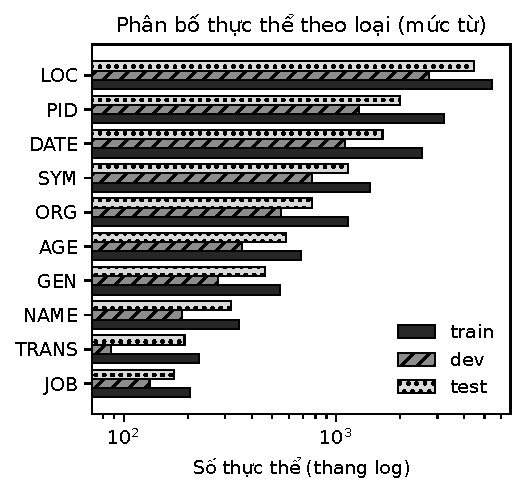
\includegraphics[width=0.98\columnwidth]{../outputs/figures/eda_entity_distribution.pdf}
\caption{Phân bố số lượng thực thể (thang logarit) của $10$ loại nhãn trên ba tập \texttt{train}, \texttt{dev} và \texttt{test}.}
\label{fig:eda_entity_dist}
\end{figure}

\begin{figure}[t]
\centering
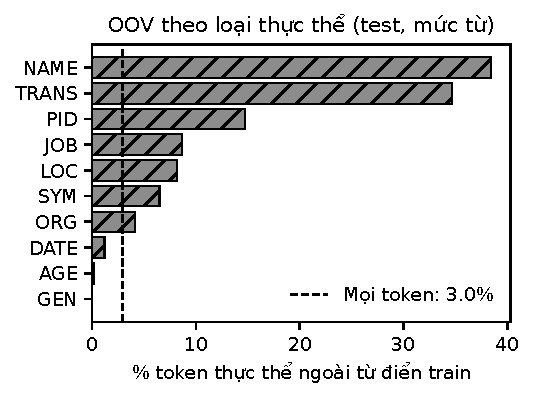
\includegraphics[width=0.98\columnwidth]{../outputs/figures/eda_oov_by_type.pdf}
\caption{Tỉ lệ phần trăm token thực thể trên tập \texttt{test\_word} chưa từng xuất hiện trong từ điển tập \texttt{train\_word} ($\text{\texttt{min\_freq}}=1$).}
\label{fig:eda_oov}
\end{figure}

Bảng~\ref{tab:data_splits}, Bảng~\ref{tab:entity_dist} cùng Hình~\ref{fig:eda_entity_dist} và Hình~\ref{fig:eda_oov} (trích xuất từ notebook EDA \texttt{01\_eda\_data\_stats.ipynb}) cho thấy bốn đặc trưng quan trọng của dữ liệu:
\begin{enumerate}
  \item \textbf{Độ dài câu vừa phải, phù hợp với giới hạn ngữ cảnh 256 của PhoBERT:} Ở mức từ, câu có độ dài trung bình $26{,}36$ từ (phân vị thứ $95$ là $50$ từ, câu dài nhất tập \texttt{train} là $161$ từ và tập \texttt{test} là $162$ từ). Ở mức âm tiết, độ dài trung bình tăng lên $33{,}33$ âm tiết (cực đại $186$ âm tiết).
  \item \textbf{Mất cân bằng lớp (\textit{class imbalance}) rất lớn:} Nhãn ngoài thực thể \texttt{O} chiếm từ $74{,}17\%$ đến $79{,}05\%$ tổng số từ. Trong $34.980$ thực thể toàn bộ dữ liệu, riêng hai loại \texttt{LOCATION} ($35{,}95\%$) và \texttt{PATIENT\_ID} ($18{,}64\%$) đã chiếm hơn một nửa, trong khi hai loại hiếm nhất là \texttt{OCCUPATION} (trong dữ liệu gán là \texttt{JOB}, $1{,}46\%$) và \texttt{TRANSPORTATION} ($1{,}45\%$) chỉ có khoảng $200$ mẫu huấn luyện mỗi loại.
  \item \textbf{Sự phân hóa về độ dài thực thể:} Các thực thể \texttt{AGE}, \texttt{GENDER}, \texttt{PATIENT\_ID} có hơn $99{,}7\%$ số mẫu chỉ dài đúng $1$ từ. Ngược lại, \texttt{ORGANIZATION} có độ dài trung bình $3{,}24$ từ ($5{,}24$ âm tiết, cực đại $14$ từ), tiếp theo là \texttt{SYMPTOM\_AND\_DISEASE} ($2{,}08$ từ), \texttt{DATE} ($1{,}98$ từ) và \texttt{LOCATION} ($1{,}97$ từ, cực đại $13$ từ). Đây là những lớp dễ phát sinh lỗi ranh giới nhất.
  \item \textbf{Tỉ lệ OOV tập trung mạnh ở thực thể định danh mới:} Với từ điển tập \texttt{train} gồm $5.169$ từ ($\text{\texttt{min\_freq}}=1$), tỉ lệ OOV chung trên toàn tập \texttt{test} chỉ là $2{,}96\%$ (tăng lên $4{,}49\%$ khi đặt $\text{\texttt{min\_freq}}=2$, kích thước từ điển còn $3.274$ từ). Tuy nhiên, nếu xét riêng các token nằm trong thực thể thì \texttt{PERSON\_NAME} có tới $38{,}4\%$ token OOV, \texttt{TRANSPORTATION} có $34{,}7\%$ và \texttt{PATIENT\_ID} có $14{,}7\%$ (Hình~\ref{fig:eda_oov}), do các ca bệnh mới, tên người mới và số hiệu chuyến bay mới xuất hiện liên tục theo thời gian. Kiểm tra tự động cũng xác nhận dữ liệu gốc có $0$ lỗi vi phạm quy tắc BIO trên cả $6$ tập.
\end{enumerate}

\subsection{Chỉ số Đánh giá (Evaluation Metrics)}
\label{sec:metrics}
Toàn bộ mô hình được đánh giá bằng thước đo \textbf{CoNLL entity-level strict match} theo lược đồ \textbf{IOB2} thông qua thư viện \texttt{seqeval} (\texttt{mode="strict", scheme=IOB2}) trên chuỗi dự đoán đã quy về mức từ gốc. Gọi $\mathcal{G}_i = \mathcal{E}(\mathbf{y}^{(i)})$ và $\mathcal{P}_i = \mathcal{E}(\hat{\mathbf{y}}^{(i)})$ lần lượt là tập thực thể chuẩn và tập thực thể dự đoán của câu thứ $i$. Một thực thể dự đoán $(c, s, e) \in \mathcal{P}_i$ chỉ được tính là một lần dự đoán đúng (\textit{True Positive} — TP) khi và chỉ khi tồn tại phần tử trùng khớp hoàn toàn cả loại nhãn lẫn chỉ số đầu--cuối $(c, s, e) \in \mathcal{G}_i$.

Với từng loại thực thể $c \in \mathcal{C}$, gọi $\text{TP}_c$, $\text{FP}_c$, $\text{FN}_c$ lần lượt là tổng số thực thể loại $c$ đoán đúng, báo nhầm và bỏ sót trên toàn bộ tập đánh giá. Độ chính xác ($\text{Precision}_c$), độ phủ ($\text{Recall}_c$) và điểm $\text{F1}_c$ được xác định bởi:
\begin{equation}
  \text{P}_c = \frac{\text{TP}_c}{\text{TP}_c + \text{FP}_c}, \quad
  \text{R}_c = \frac{\text{TP}_c}{\text{TP}_c + \text{FN}_c}, \quad
  \text{F1}_c = \frac{2 \text{P}_c \text{R}_c}{\text{P}_c + \text{R}_c}.
\end{equation}
Từ đó, chúng tôi báo cáo hai chỉ số tổng hợp chính:
\begin{itemize}
  \item \textbf{Micro-F1:} Gộp tổng $\text{TP} = \sum_{c} \text{TP}_c$, $\text{FP} = \sum_{c} \text{FP}_c$, $\text{FN} = \sum_{c} \text{FN}_c$ trước khi tính F1. Chỉ số này phản ánh hiệu năng tổng thể trên mọi thực thể nhưng chịu ảnh hưởng lớn bởi các lớp đa số (\texttt{LOCATION}, \texttt{PATIENT\_ID}).
  \item \textbf{Macro-F1:} Trung bình cộng không trọng số $\text{Macro-F1} = \frac{1}{|\mathcal{C}|} \sum_{c \in \mathcal{C}} \text{F1}_c$, đặt trọng số ngang nhau cho cả $10$ loại thực thể nên đánh giá nhạy bén khả năng nhận diện các lớp thiểu số (\texttt{JOB}, \texttt{TRANSPORTATION}, \texttt{NAME}).
  \item \textbf{Số vi phạm ràng buộc BIO ($\text{BIO-Viol}$):} Đếm tổng số vị trí token dự đoán $\hat{y}_t = \text{\texttt{I-}}c$ không đứng ngay sau $\text{\texttt{B-}}c$ hoặc $\text{\texttt{I-}}c$ cùng loại. Trong chế độ \texttt{strict IOB2}, một chuỗi dự đoán bất hợp lệ như \texttt{[O, I-LOCATION]} không tạo thành thực thể hợp lệ nào và bị phạt trực tiếp vào Recall.
\end{itemize}

\subsection{Thiết lập Huấn luyện và Kết quả Chính}
\label{sec:main_results}
Các thí nghiệm được huấn luyện trên hạ tầng GPU đám mây Kaggle (NVIDIA Tesla T4 / P100 16GB VRAM) và Google Colab (T4 16GB VRAM), cố định \texttt{seed = 42} trên mọi thư viện (\texttt{random}, \texttt{numpy}, \texttt{torch}) và ghi nhận log trực tuyến qua Weights \& Biases (\texttt{wandb}). Thời gian huấn luyện trung bình của \texttt{BiLSTM-CRF} là \texttt{[CHỜ SỐ LIỆU: Thời gian train BiLSTM-CRF]} phút và của \texttt{PhoBERT} là \texttt{[CHỜ SỐ LIỆU: Thời gian train PhoBERT]} phút.

% Nhúng Bảng 1 (Kết quả chính) và Bảng 2 (F1 theo 10 loại thực thể) được sinh tự động bởi scripts/export_latex_tables.py
\begin{table*}[t]
\centering
\small
\begin{tabular}{lccccc}
\hline
\textbf{Mô hình} & \textbf{Micro-P (\%)} & \textbf{Micro-R (\%)} & \textbf{Micro-F1 (\%)} & \textbf{Macro-F1 (\%)} & \textbf{Vi phạm BIO} \\
\hline
BiLSTM + CharCNN + CRF (From Scratch) & [CHỜ SỐ LIỆU: BiLSTM + CharCNN + CRF (From Scratch) Micro-P] & [CHỜ SỐ LIỆU: BiLSTM + CharCNN + CRF (From Scratch) Micro-R] & [CHỜ SỐ LIỆU: BiLSTM + CharCNN + CRF (From Scratch) Micro-F1] & [CHỜ SỐ LIỆU: BiLSTM + CharCNN + CRF (From Scratch) Macro-F1] & [CHỜ SỐ LIỆU: BiLSTM + CharCNN + CRF (From Scratch) BIO] \\
PhoBERT-base-v2 Fine-tune & [CHỜ SỐ LIỆU: PhoBERT-base-v2 Fine-tune Micro-P] & [CHỜ SỐ LIỆU: PhoBERT-base-v2 Fine-tune Micro-R] & [CHỜ SỐ LIỆU: PhoBERT-base-v2 Fine-tune Micro-F1] & [CHỜ SỐ LIỆU: PhoBERT-base-v2 Fine-tune Macro-F1] & [CHỜ SỐ LIỆU: PhoBERT-base-v2 Fine-tune BIO] \\
\hline
\end{tabular}
\caption{Kết quả đánh giá tổng thể mức thực thể (strict IOB2) trên tập \texttt{test} của PhoNER\_COVID19.}
\label{tab:main_results}
\end{table*}

\begin{table}[t]
\centering
\small
\begin{tabular}{lrcc}
\hline
\textbf{Loại thực thể} & \textbf{Số lượng} & \textbf{BiLSTM-CRF} & \textbf{PhoBERT} \\
\hline
AGE (\texttt{AGE}) & 582 & [CHỜ SỐ LIỆU: F1 AGE (BiLSTM-CRF)] & [CHỜ SỐ LIỆU: F1 AGE (PhoBERT)] \\
DATE (\texttt{DATE}) & 1654 & [CHỜ SỐ LIỆU: F1 DATE (BiLSTM-CRF)] & [CHỜ SỐ LIỆU: F1 DATE (PhoBERT)] \\
GENDER (\texttt{GEN}) & 462 & [CHỜ SỐ LIỆU: F1 GENDER (BiLSTM-CRF)] & [CHỜ SỐ LIỆU: F1 GENDER (PhoBERT)] \\
OCCUPATION (\texttt{JOB}) & 173 & [CHỜ SỐ LIỆU: F1 OCCUPATION (BiLSTM-CRF)] & [CHỜ SỐ LIỆU: F1 OCCUPATION (PhoBERT)] \\
LOCATION (\texttt{LOC}) & 4441 & [CHỜ SỐ LIỆU: F1 LOCATION (BiLSTM-CRF)] & [CHỜ SỐ LIỆU: F1 LOCATION (PhoBERT)] \\
PERSON\_NAME (\texttt{NAME}) & 318 & [CHỜ SỐ LIỆU: F1 PERSON\_NAME (BiLSTM-CRF)] & [CHỜ SỐ LIỆU: F1 PERSON\_NAME (PhoBERT)] \\
ORGANIZATION (\texttt{ORG}) & 771 & [CHỜ SỐ LIỆU: F1 ORGANIZATION (BiLSTM-CRF)] & [CHỜ SỐ LIỆU: F1 ORGANIZATION (PhoBERT)] \\
PATIENT\_ID (\texttt{PID}) & 2005 & [CHỜ SỐ LIỆU: F1 PATIENT\_ID (BiLSTM-CRF)] & [CHỜ SỐ LIỆU: F1 PATIENT\_ID (PhoBERT)] \\
SYMPTOM\_AND\_DISEASE (\texttt{SYM}) & 1136 & [CHỜ SỐ LIỆU: F1 SYMPTOM\_AND\_DISEASE (BiLSTM-CRF)] & [CHỜ SỐ LIỆU: F1 SYMPTOM\_AND\_DISEASE (PhoBERT)] \\
TRANSPORTATION (\texttt{TRANS}) & 193 & [CHỜ SỐ LIỆU: F1 TRANSPORTATION (BiLSTM-CRF)] & [CHỜ SỐ LIỆU: F1 TRANSPORTATION (PhoBERT)] \\
\hline
\textbf{Micro-F1} & — & [CHỜ SỐ LIỆU: Micro-F1 (BiLSTM-CRF)] & [CHỜ SỐ LIỆU: Micro-F1 (PhoBERT)] \\
\textbf{Macro-F1} & — & [CHỜ SỐ LIỆU: Macro-F1 (BiLSTM-CRF)] & [CHỜ SỐ LIỆU: Macro-F1 (PhoBERT)] \\
\hline
\end{tabular}
\caption{Điểm F1 (\%) theo từng loại thực thể trên tập \texttt{test}.}
\label{tab:per_entity_f1}
\end{table}


Bảng~\ref{tab:main_results} trình bày kết quả đối sánh tổng thể trên tập \texttt{test\_word}, và Bảng~\ref{tab:per_entity_f1} chi tiết hóa điểm F1 trên từng loại trong $10$ loại thực thể. Khi có đầy đủ kết quả huấn luyện từ hai nhánh mô hình, bảng số liệu được cập nhật tự động thông qua script \texttt{python scripts/export\_latex\_tables.py} từ các tệp \texttt{outputs/metrics/*.json}.

% =============================================================================
\section{Phân tích Chuyên sâu (Analysis)}
\label{sec:analysis}

\subsection{Nghiên cứu Cắt bỏ (Ablation Study)}
\label{sec:ablation}
Để tách biệt đóng góp của từng thành phần kiến trúc, nhóm thực hiện hai nhóm thí nghiệm cắt bỏ có kiểm soát trên cùng tập \texttt{test\_word} (Bảng~\ref{tab:ablation_bilstm} và Bảng~\ref{tab:ablation_phobert}):
\begin{enumerate}
  \item \textbf{Trên \texttt{BiLSTM-CRF}:} (i) Mô hình đầy đủ \texttt{BiLSTM + CharCNN + CRF}; (ii) Loại bỏ nhánh biểu diễn ký tự \texttt{CharCNN} (chỉ dùng \texttt{WordEmbedding + BiLSTM + CRF}); và (iii) Loại bỏ tầng \texttt{Linear-chain CRF}, thay bằng tầng phân loại độc lập \texttt{Linear + Softmax} tối ưu qua \texttt{CrossEntropyLoss}.
  \item \textbf{Trên \texttt{PhoBERT}:} (i) Tinh chỉnh toàn bộ tham số (\textit{full fine-tune}) với tầng ẩn cuối và đầu Softmax; (ii) Nối $4$ tầng ẩn cuối của Transformer (\textit{concat last-4 layers}); (iii) Thay đầu Softmax bằng tầng \texttt{Linear-chain CRF} tự cài của dự án trên chuỗi vector subword đầu tiên; và (iv) Đóng băng toàn bộ trọng số \texttt{PhoBERT} (\textit{freeze backbone}), chỉ huấn luyện tầng phân loại tuyến tính phía trên.
\end{enumerate}

\begin{table}[t]
\centering
\small
\begin{tabular}{lcccc}
\hline
\textbf{Cấu hình} & \textbf{Micro-F1} & \textbf{Macro-F1} & \textbf{$\Delta$F1} & \textbf{Lỗi BIO} \\
\hline
BiLSTM + CharCNN + CRF (Đầy đủ) & [CHỜ SỐ LIỆU: BiLSTM + CharCNN + CRF (Đầy đủ) Micro-F1] & [CHỜ SỐ LIỆU: BiLSTM + CharCNN + CRF (Đầy đủ) Macro-F1] & — & [CHỜ SỐ LIỆU: BiLSTM + CharCNN + CRF (Đầy đủ) BIO] \\
  \$-\$ Character Embedding (BiLSTM + CRF) & [CHỜ SỐ LIỆU:   \$-\$ Character Embedding (BiLSTM + CRF) Micro-F1] & [CHỜ SỐ LIỆU:   \$-\$ Character Embedding (BiLSTM + CRF) Macro-F1] & — & [CHỜ SỐ LIỆU:   \$-\$ Character Embedding (BiLSTM + CRF) BIO] \\
  \$-\$ Tầng CRF (BiLSTM + CharCNN + Softmax) & [CHỜ SỐ LIỆU:   \$-\$ Tầng CRF (BiLSTM + CharCNN + Softmax) Micro-F1] & [CHỜ SỐ LIỆU:   \$-\$ Tầng CRF (BiLSTM + CharCNN + Softmax) Macro-F1] & — & [CHỜ SỐ LIỆU:   \$-\$ Tầng CRF (BiLSTM + CharCNN + Softmax) BIO] \\
\hline
\end{tabular}
\caption{Ablation Study cho mô hình BiLSTM-CRF tự cài đặt.}
\label{tab:ablation_bilstm}
\end{table}

\begin{table}[t]
\centering
\small
\begin{tabular}{lcccc}
\hline
\textbf{Cấu hình} & \textbf{Micro-F1} & \textbf{Macro-F1} & \textbf{$\Delta$F1} & \textbf{Lỗi BIO} \\
\hline
PhoBERT Full Fine-tune + Last Layer + Softmax & [CHỜ SỐ LIỆU: PhoBERT Full Fine-tune + Last Layer + Softmax Micro-F1] & [CHỜ SỐ LIỆU: PhoBERT Full Fine-tune + Last Layer + Softmax Macro-F1] & — & [CHỜ SỐ LIỆU: PhoBERT Full Fine-tune + Last Layer + Softmax BIO] \\
  $+$ Nối 4 tầng ẩn cuối (Concat Last-4) & [CHỜ SỐ LIỆU:   \$+\$ Nối 4 tầng ẩn cuối (Concat Last-4) Micro-F1] & [CHỜ SỐ LIỆU:   \$+\$ Nối 4 tầng ẩn cuối (Concat Last-4) Macro-F1] & — & [CHỜ SỐ LIỆU:   \$+\$ Nối 4 tầng ẩn cuối (Concat Last-4) BIO] \\
  $+$ Tầng Linear-chain CRF (PhoBERT + CRF) & [CHỜ SỐ LIỆU:   \$+\$ Tầng Linear-chain CRF (PhoBERT + CRF) Micro-F1] & [CHỜ SỐ LIỆU:   \$+\$ Tầng Linear-chain CRF (PhoBERT + CRF) Macro-F1] & — & [CHỜ SỐ LIỆU:   \$+\$ Tầng Linear-chain CRF (PhoBERT + CRF) BIO] \\
  $-$ Đóng băng Backbone (Freeze PhoBERT) & [CHỜ SỐ LIỆU:   \$-\$ Đóng băng Backbone (Freeze PhoBERT) Micro-F1] & [CHỜ SỐ LIỆU:   \$-\$ Đóng băng Backbone (Freeze PhoBERT) Macro-F1] & — & [CHỜ SỐ LIỆU:   \$-\$ Đóng băng Backbone (Freeze PhoBERT) BIO] \\
\hline
\end{tabular}
\caption{Ablation Study cho mô hình PhoBERT fine-tune.}
\label{tab:ablation_phobert}
\end{table}


\subsection{Phân tích Vi phạm Ràng buộc BIO và Vai trò của Tầng CRF}
\label{sec:bio_analysis}
Một câu hỏi cốt lõi khi bảo vệ phương pháp là: \textit{``Tại sao cần tầng CRF với độ phức tạp $O(N|\mathcal{Y}|^2)$ trong khi BiLSTM đã nhìn thấy ngữ cảnh hai chiều?''} Câu trả lời nằm ở sự khác biệt giữa ngữ cảnh của đặc trưng đầu vào ($\mathbf{h}_t$) và sự phụ thuộc trực tiếp giữa các quyết định nhãn đầu ra ($y_{t-1} \to y_t$). Khi dùng đầu dự đoán Softmax, xác suất tại mỗi vị trí $P(y_t \mid \mathbf{h}_t)$ được chọn độc lập bằng $\arg\max$, dẫn tới việc mô hình có thể sinh ra các nhãn \texttt{I-}$c$ đứng cô lập sau nhãn \texttt{O} hoặc nối đuôi một thực thể khác loại $\text{\texttt{B-}}c'$ ($c' \ne c$).

Trên tập \texttt{test\_word}, mô hình không dùng CRF phát sinh \texttt{[CHỜ SỐ LIỆU: Số lỗi BIO của BiLSTM-Softmax]} nhãn vi phạm BIO trên \texttt{[CHỜ SỐ LIỆU: Số câu lỗi BIO của BiLSTM-Softmax]} câu, trong khi mô hình có tầng \texttt{Linear-chain CRF} giảm số vi phạm xuống \texttt{[CHỜ SỐ LIỆU: Số lỗi BIO của BiLSTM-CRF]} nhờ ma trận chuyển trạng thái $\mathbf{A}$ học được trọng số âm lớn tại các cặp chuyển nhãn phi lý ($\text{\texttt{O}} \to \text{\texttt{I-}}c$ và $\text{\texttt{B-}}c' \to \text{\texttt{I-}}c$). Hơn nữa, khi thử áp dụng hàm hậu xử lý \texttt{repair\_bio} (chuyển các nhãn \texttt{I-}$c$ mồ côi thành \texttt{B-}$c$), Micro-F1 của mô hình Softmax thay đổi từ \texttt{[CHỜ SỐ LIỆU: Micro-F1 BiLSTM-Softmax trước sửa BIO]}\% lên \texttt{[CHỜ SỐ LIỆU: Micro-F1 BiLSTM-Softmax sau sửa BIO]}\%, nhưng vẫn thấp hơn \texttt{BiLSTM-CRF} do CRF tìm đường đi tối ưu toàn cục bằng Viterbi thay vì chỉ sửa cục bộ từng điểm gãy.

\subsection{Phân loại 4 Nhóm Lỗi Thực thể, Độ dài và OOV}
\label{sec:error_taxonomy}
Để hiểu bản chất các ca dự đoán sai thay vì chỉ nhìn vào một con số F1 tổng hợp, module \texttt{src/evaluation/error\_analysis.py} đối chiếu tập thực thể chuẩn $\mathcal{G}_i$ và tập dự đoán $\mathcal{P}_i$ trên từng câu (sau khi loại bỏ các thực thể khớp tuyệt đối) và phân chia mọi sai số vào đúng bốn nhóm loại trừ lẫn nhau:
\begin{enumerate}
  \item \textbf{Lỗi ranh giới (\textit{Boundary Error}):} Thực thể dự đoán $(c, s', e')$ có phần giao khác rỗng với một thực thể chuẩn $(c, s, e)$ \textbf{cùng loại} $c$, nhưng lệch điểm bắt đầu hoặc kết thúc ($(s', e') \ne (s, e)$). Ví dụ: nhãn chuẩn là \texttt{[Bệnh\_viện Đà\_Nẵng]\textsubscript{LOC}} nhưng mô hình chỉ bắt được \texttt{[Đà\_Nẵng]\textsubscript{LOC}}.
  \item \textbf{Lỗi nhầm loại (\textit{Type Error}):} Thực thể dự đoán $(c', s', e')$ giao với thực thể chuẩn $(c, s, e)$ nhưng \textbf{khác loại} ($c' \ne c$). Cặp nhầm lẫn phổ biến nhất là giữa \texttt{LOCATION} và \texttt{ORGANIZATION} trên các cơ sở y tế/hành chính, hoặc giữa \texttt{PATIENT\_ID} và \texttt{AGE} trên các con số đứng gần nhau.
  \item \textbf{Lỗi báo nhầm (\textit{False Positive — FP}):} Mô hình sinh ra một thực thể trên vùng toàn nhãn \texttt{O} của nhãn chuẩn (không giao với bất kỳ thực thể chuẩn nào).
  \item \textbf{Lỗi bỏ sót (\textit{False Negative — FN}):} Thực thể chuẩn bị dự đoán thành toàn nhãn \texttt{O} (không có thực thể dự đoán nào chạm tới).
\end{enumerate}

\begin{table}[t]
\centering
\small
\begin{tabular}{lcc}
\hline
\textbf{Nhóm lỗi / Chỉ số phân tích} & \textbf{BiLSTM-CRF} & \textbf{PhoBERT} \\
\hline
Thực thể đoán đúng hoàn toàn (TP) & \texttt{[CHỜ SỐ LIỆU: TP BiLSTM-CRF]} & \texttt{[CHỜ SỐ LIỆU: TP PhoBERT]} \\
1. Lỗi ranh giới (\textit{Boundary}) & \texttt{[CHỜ SỐ LIỆU: Boundary BiLSTM-CRF]} & \texttt{[CHỜ SỐ LIỆU: Boundary PhoBERT]} \\
2. Lỗi nhầm loại (\textit{Type}) & \texttt{[CHỜ SỐ LIỆU: Type BiLSTM-CRF]} & \texttt{[CHỜ SỐ LIỆU: Type PhoBERT]} \\
3. Báo nhầm (\textit{False Positive}) & \texttt{[CHỜ SỐ LIỆU: FP BiLSTM-CRF]} & \texttt{[CHỜ SỐ LIỆU: FP PhoBERT]} \\
4. Bỏ sót (\textit{False Negative}) & \texttt{[CHỜ SỐ LIỆU: FN BiLSTM-CRF]} & \texttt{[CHỜ SỐ LIỆU: FN PhoBERT]} \\
\hline
Recall thực thể toàn từ đã biết (\%) & \texttt{[CHỜ SỐ LIỆU: Recall Known BiLSTM-CRF]} & \texttt{[CHỜ SỐ LIỆU: Recall Known PhoBERT]} \\
Recall thực thể chứa từ OOV (\%) & \texttt{[CHỜ SỐ LIỆU: Recall OOV BiLSTM-CRF]} & \texttt{[CHỜ SỐ LIỆU: Recall OOV PhoBERT]} \\
Recall thực thể dài $\ge 4$ từ (\%) & \texttt{[CHỜ SỐ LIỆU: Recall Len>=4 BiLSTM-CRF]} & \texttt{[CHỜ SỐ LIỆU: Recall Len>=4 PhoBERT]} \\
\hline
\end{tabular}
\caption{Thống kê phân rã $4$ nhóm lỗi thực thể và độ phủ (Recall) theo tính chất từ vựng OOV / độ dài thực thể trên tập \texttt{test\_word}.}
\label{tab:error_breakdown}
\end{table}

\begin{table*}[t]
\centering
\small
\begin{tabular}{p{2.5cm}p{6.2cm}p{6.2cm}}
\hline
\textbf{Loại hiện tượng} & \textbf{Chuỗi nhãn chuẩn (Gold) / Nhận xét} & \textbf{Dự đoán của mô hình} \\
\hline
Lỗi ranh giới (\textit{Boundary}) trên thực thể dài &
\textit{Gold:} \texttt{... điều\_trị tại [Bệnh\_viện Bệnh\_nhiệt\_đới Trung\_ương cơ\_sở Đông\_Anh]\textsubscript{LOC} .}\newline
Thực thể gồm $6$ từ ghép nối tiếp chỉ cơ sở điều trị kèm địa danh hành chính. &
\texttt{[CHỜ SỐ LIỆU: Ví dụ dự đoán Boundary thật từ error\_samples\_bilstm.csv]} (Mô hình thường cắt sớm sau cụm danh từ chính hoặc tách phần địa danh phía sau thành thực thể rời). \\
\hline
Lỗi nhầm loại (\textit{Type}) \texttt{LOC} $\leftrightarrow$ \texttt{ORG} &
\textit{Gold:} \texttt{... theo thông\_báo của [Bệnh\_viện Đà\_Nẵng]\textsubscript{ORG} , bệnh\_nhân từng đến [Bệnh\_viện Đà\_Nẵng]\textsubscript{LOC} .}\newline
Cùng một bề mặt từ vựng nhưng đóng hai vai trò ngữ nghĩa khác nhau theo giới từ đứng trước. &
\texttt{[CHỜ SỐ LIỆU: Ví dụ dự đoán Type thật từ error\_samples\_bilstm.csv]} (\texttt{PhoBERT} phân biệt tốt hơn nhờ cơ chế Self-Attention toàn câu bắt được động từ/giới từ điều khiển). \\
\hline
Thực thể chứa từ OOV (\texttt{NAME}, \texttt{TRANS}) &
\textit{Gold:} \texttt{... hành\_khách [N.T.H.]\textsubscript{NAME} trên chuyến bay [QH152]\textsubscript{TRANS} ...}\newline
Các token \texttt{N.T.H.} và \texttt{QH152} không xuất hiện trong tập \texttt{train}. &
\texttt{[CHỜ SỐ LIỆU: Ví dụ dự đoán OOV thật]} (Nhánh \texttt{CharCNN} và BPE subword giúp nhận diện mẫu chữ cái viết hoa kèm dấu chấm/chữ số thay vì suy biến thành vector \texttt{<unk>} vô hướng). \\
\hline
\end{tabular}
\caption{Khung phân tích định tính các trường hợp dự đoán điển hình theo từng nhóm thách thức trên \texttt{PhoNER\_COVID19}.}
\label{tab:qualitative_examples}
\end{table*}

Bảng~\ref{tab:error_breakdown} và Bảng~\ref{tab:qualitative_examples} tổng hợp bức tranh định lượng và định tính từ notebook \texttt{04\_error\_analysis.ipynb}. Toàn bộ biểu đồ trực quan hóa (F1 theo từng thực thể, ma trận nhầm lẫn chuẩn hóa theo hàng của hai mô hình, biểu đồ 4 nhóm lỗi, biểu đồ vi phạm BIO và đường cong Recall theo độ dài thực thể) được xuất tự động ở định dạng vector thang xám (\texttt{outputs/figures/eval\_*.pdf}) để chèn trực tiếp ngay khi hoàn tất lượt chạy huấn luyện cuối.

% =============================================================================
\section{Kết luận (Conclusion)}
\label{sec:conclusion}
Báo cáo đã xây dựng một quy trình thực nghiệm hoàn chỉnh, minh bạch và có khả năng tái lập cao cho bài toán Nhận dạng thực thể có tên tiếng Việt trên bộ dữ liệu \texttt{PhoNER\_COVID19}. Bằng việc tự cài đặt từ đầu kiến trúc \texttt{BiLSTM-CRF} có tầng nhúng ký tự và đặt trong phép so sánh trực tiếp với mô hình ngôn ngữ tiền huấn luyện \texttt{PhoBERT} trên cùng một bộ chấm điểm \texttt{seqeval} strict IOB2 mức từ, nghiên cứu làm rõ vai trò bổ trợ giữa ràng buộc cấu trúc nhãn đầu ra (CRF) và biểu diễn ngữ cảnh sâu (Transformer). Trong tương lai, kiến trúc giao diện dự đoán đã chốt của dự án cho phép mở rộng trực tiếp sang thực nghiệm đối sánh mức âm tiết (\texttt{syllable-level}) và đánh giá khả năng học ít mẫu (\textit{few-shot in-context learning}) của các mô hình ngôn ngữ lớn (LLM).

% =============================================================================
% Các mục bên dưới không tính vào giới hạn 8 trang nội dung theo quy định ACL và đề bài.
\section*{Giới hạn của Nghiên cứu (Limitations)}
\label{sec:limitations}

\paragraph{1. Giới hạn từ đặc trưng dữ liệu và tiền xử lý tách từ.}
Bộ dữ liệu \texttt{PhoNER\_COVID19} có độ lệch phân bố lớp rất lớn: hai lớp hiếm \texttt{OCCUPATION} ($205$ mẫu train) và \texttt{TRANSPORTATION} ($226$ mẫu train) có kích thước nhỏ hơn lớp \texttt{LOCATION} tới hơn $24$ lần, khiến phương sai ước lượng F1 trên các lớp thiểu số cao hơn đáng kể. Bên cạnh đó, dữ liệu mức từ (\texttt{word-level}) phụ thuộc chặt vào bộ tách từ tiếng Việt ở bước tiền xử lý: trong thực tế triển khai (như trên ứng dụng Demo Gradio khi người dùng nhập văn bản thô), nếu bộ tách từ (\texttt{Underthesea}/\texttt{VnCoreNLP}) ghép sai ranh giới một từ nằm ở biên thực thể, mô hình gán nhãn mức từ không thể tự khôi phục ranh giới âm tiết bên trong từ ghép đó. Ngoài ra, dữ liệu thu thập từ tin tức dịch tễ giai đoạn 2020--2021 nên từ vựng mang tính thời điểm; khi áp dụng sang bệnh án điện tử lâm sàng hoặc tin tức y tế tổng quát, hiện tượng dịch chuyển miền (\textit{domain shift}) là không tránh khỏi.

\paragraph{2. Giới hạn của thước đo đánh giá nghiêm ngặt (\textit{Strict Evaluation}).}
Thước đo \texttt{seqeval} ở chế độ \texttt{strict IOB2} đòi hỏi khớp tuyệt đối cả loại thực thể lẫn vị trí token đầu--cuối. Trong thước đo này, một dự đoán bắt được $5/6$ từ của một thực thể \texttt{LOCATION} dài vẫn bị tính đồng thời là $1$ lỗi False Positive và $1$ lỗi False Negative — tức bị phạt nặng hơn cả việc mô hình dự đoán toàn nhãn \texttt{O} (chỉ chịu $1$ lỗi False Negative). Chính vì hạn chế này của chỉ số F1 đơn lẻ, chúng tôi đã bổ sung phân rã $4$ nhóm lỗi trong Mục~\ref{sec:error_taxonomy} để tách bạch lỗi lệch ranh giới một phần khỏi lỗi bỏ sót hoàn toàn.

\paragraph{3. Giới hạn về tài nguyên tính toán.}
Do giới hạn thời gian phiên chạy trên GPU miễn phí của Kaggle và Google Colab, nhóm chưa thực hiện tìm kiếm lưới siêu tham số toàn diện (\textit{exhaustive grid search}) trên nhiều hạt giống ngẫu nhiên (\textit{multi-seed runs}) để báo cáo độ lệch chuẩn của từng cấu hình ablation.

\section*{Đóng góp của Thành viên và Khai báo Công cụ AI}
\label{sec:contributions}

\begin{table}[h]
\centering
\small
\begin{tabular}{p{1.5cm}p{4.6cm}c}
\hline
\textbf{Thành viên} & \textbf{Phân hệ phụ trách chính} & \textbf{Tỉ lệ} \\
\hline
\textbf{Đạt} &
Thiết kế Hợp đồng giao diện; cài đặt toàn bộ Data Pipeline (\texttt{download.py}, \texttt{labels.py}, \texttt{vocab.py}, \texttt{bilstm\_dataset.py}); EDA (\texttt{01\_eda\_data\_stats.ipynb}); bộ chấm điểm chuẩn \& kiểm tra BIO (\texttt{metrics.py}, \texttt{predictions.py}); phân tích 4 nhóm lỗi \& trực quan hóa thang xám (\texttt{error\_analysis.py}, \texttt{plots.py}, \texttt{04\_error\_analysis.ipynb}); tự động xuất bảng LaTeX (\texttt{latex\_tables.py}); bộ Unit Test (\texttt{tests/}); ứng dụng Demo Gradio (\texttt{app/}); viết mục Introduction, Dữ liệu, Chỉ số đánh giá, Analysis, Limitations và tổng hợp báo cáo. &
$33{,}3\%$ \\
\hline
\textbf{Tín} &
Tự cài đặt từ đầu tầng \texttt{CharEncoder} (\texttt{char\_encoder.py}), tầng \texttt{Linear-chain CRF} với thuật toán Forward--Viterbi \& \texttt{log\_sum\_exp} có xử lý \texttt{mask} (\texttt{crf.py}), kiến trúc tích hợp \texttt{BiLSTM-CRF} (\texttt{bilstm\_crf.py}); huấn luyện và chạy Ablation Study cho nhánh BiLSTM-CRF trên Kaggle/Colab (\texttt{02\_train\_bilstm\_crf.ipynb}); viết mục Phương pháp \& Thí nghiệm BiLSTM-CRF. &
$33{,}3\%$ \\
\hline
\textbf{Đức Anh} &
Cài đặt xử lý BPE subword \& First-Subword Alignment cho PhoBERT (\texttt{phobert\_dataset.py}); kiến trúc \texttt{PhoBERT} fine-tuning với Differential LR, nối 4 tầng ẩn cuối và tùy chọn ghép tầng CRF (\texttt{phobert\_ner.py}); huấn luyện và chạy Ablation Study cho nhánh PhoBERT (\texttt{03\_train\_phobert.ipynb}); viết mục Related Work, Phương pháp \& Thí nghiệm PhoBERT. &
$33{,}3\%$ \\
\hline
\end{tabular}
\caption{Bảng phân công công việc và tỉ lệ đóng góp của $3$ thành viên trong nhóm.}
\label{tab:member_contrib}
\end{table}

\paragraph{Khai báo sử dụng công cụ AI (AI Usage Declaration).}
Tuân thủ quy định về liêm chính học thuật của môn Học sâu, nhóm khai báo việc sử dụng công cụ trợ lý AI trong quá trình thực hiện bài tập lớn như sau:
\begin{itemize}
  \item \textbf{Phạm vi hỗ trợ:} Công cụ AI được sử dụng để hỗ trợ khởi tạo khung mã nguồn theo thiết kế mô-đun của nhóm (\textit{boilerplate code}), viết kịch bản kiểm thử đơn vị (\texttt{pytest}), tự động hóa script chuyển đổi tệp kết quả \texttt{.json} sang bảng LaTeX chuẩn ACL và rà soát lỗi chính tả/định dạng tài liệu LaTeX.
  \item \textbf{Kiểm chứng và chịu trách nhiệm:} Toàn bộ thuật toán cốt lõi, logic xử lý mặt nạ (\textit{masking}), quy tắc căn chỉnh nhãn, công thức tính chỉ số đánh giá và số liệu thống kê trong báo cáo đều được các thành viên trực tiếp kiểm tra chéo bằng unit test trên dữ liệu thật của \texttt{PhoNER\_COVID19}. Không có bất kỳ con số thực nghiệm hoặc tài liệu trích dẫn nào được sinh tự động bởi AI; mọi thành viên hiểu rõ từng dòng code trong kho mã nguồn để bảo vệ vấn đáp cá nhân.
\end{itemize}

\bibliography{references}

\end{document}
